The main result of this paper is that we can approximate $\bn_{MAP}$ in \emph{linear} time, whereas an exact solution would require exponential time. Fig. \ref{fig:wiener} shows two examples of running the FAND filter on simulated data.  On the left, the data is simulated according to Eqs. \eqref{eq:F} and \eqref{eq:C}, with a low expected firing rate (5 Hz).  The FAND filter performs very well (middle left panel): when spikes occured (gray downward facing triangles), the FAND filter's output is relatively high, and in the absence of a spike, the FAND filter's output is relatively low. The height of the ``spikes'' in $\bn_{FAND}$ can be thought of as the probability of a spike having occurred.  The Wiener filter does not perform as well on this data.  Specifically, $\bn_{Wiener}$ exhibits a ``ringing'' effect, in which the inference oscillates around zero in the absence of true spikes.  This occurs because negative spikes improve the inference, if negative spikes are allowed.  By constraining our inference to be non-negative (for the FAND filter), we completely circumvent this problem.  

It is unsurprising that the FAND filter significantly outperforms the Wiener filter when spiking is sparse, given that the exponential is a much better approximation to the Poisson in this regime (c.f. Figure \ref{fig:dist_comp}).  However, even in the fast firing rate scenario, where the Gaussian approximation is far more accurate, the FAND filter performs relatively well, as depicted in the right panels of Figure \ref{fig:wiener}.  Note however that the computational time for computing the FAND filter scales linearly with $T$, i.e. is $O(T)$, whereas the \nai ve implementation of the Wiener filter requires $O(T \log T)$ (but see Appendix \ref{sec:app} for an implementation of the Wiener for that only requires $O(T)$).  

\begin{figure}[H]
\centering 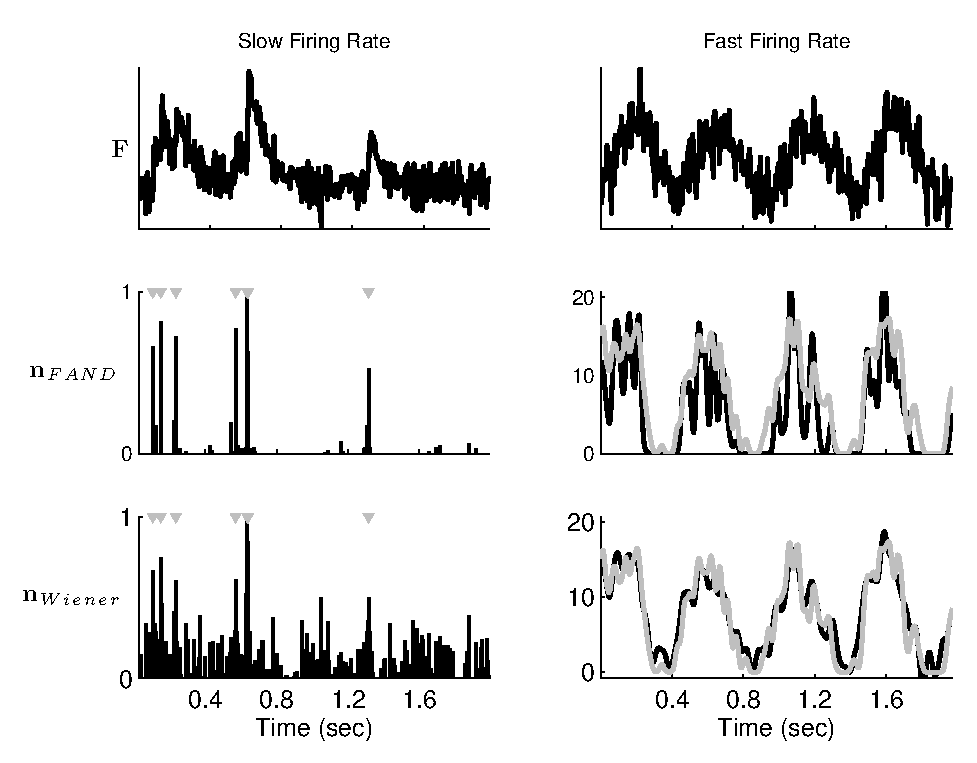
\includegraphics[width=.9\linewidth]{../figs/example_sim}
\caption{A simulation demonstrating that the FAND filter performs at least as well as the optimal linear (i.e., Wiener) filter. The left panels show that in the slow firing regime, the FAND filter outperforms the Wiener filter in terms of SNR.  This ``makes sense'', given that if a neuron is spiking according to a Poisson distribution with a slow rate, an exponential distribution is a better approximation than a Gaussian distribution, and the FAND filter approximates the spike train distribution with an exponential, versus the Wiener filter's Gaussian. The right panels show that both approximations are sufficient in the fast firing regime. Top left panel: fluorescence time series for a neuron with a slow firing rate.  Middle left panel: the FAND filter's inferred spike train.  Bottom left panel: Wiener filter's inferred spike train.  Note that (i) the Wiener filter does not impose a non-negativity constraint, and (ii) the effective SNR of the Wiener filter in this example is worse than the FAND filter's.  Top right panel: same as top left panel, for a neuron with a high firing rate.  Middle right panel: the FAND filter's inferred spike train smoothed with a Gaussian kernel for visualization purposes (black line), and the true spike train smoothed with the same Gaussian kernel (gray line).  Bottom right panel: same as middle right panel, but with the Wiener filter. Parameters for left panels: same as above.  Parameters for right panels: same as above, except: $\sig=8$ photons, $\lam=500$ Hz.} \label{fig:wiener}
\end{figure}

To quantify the relative quality of these inference algorithms in the sparsely spiking regime, we compute a number of distance measures between $\bn$ and our inferred $\hbn$: (a) cross correlation, (b) mean square error, and (c) signal-to-noise ratio (see Section \ref{sec:ass} for details). Figure \ref{fig:stats} (top panels) shows how the various algorithms (FAND in blue, Wiener in red, half-wave-rectified Wiener in green, dF/F in turquise) perform according to each of these measures, as a function of the noisiness of the data. Clearly, regardless of the variance of the noise, the FAND filter outperforms all other approaches considered here.   On the contrary, in the high firing rate regime, the Wiener filter is optimal, as expected (lower left panels).  Note that SNR is only an appropriate measure when there is at most one spike per image frame.  Finally, do demonstrate that our algorithms are indeed linear in the number of time steps, we show how computational time scales with $T$ (lower right panel) for each algorithm.


\begin{figure}[H]
\centering 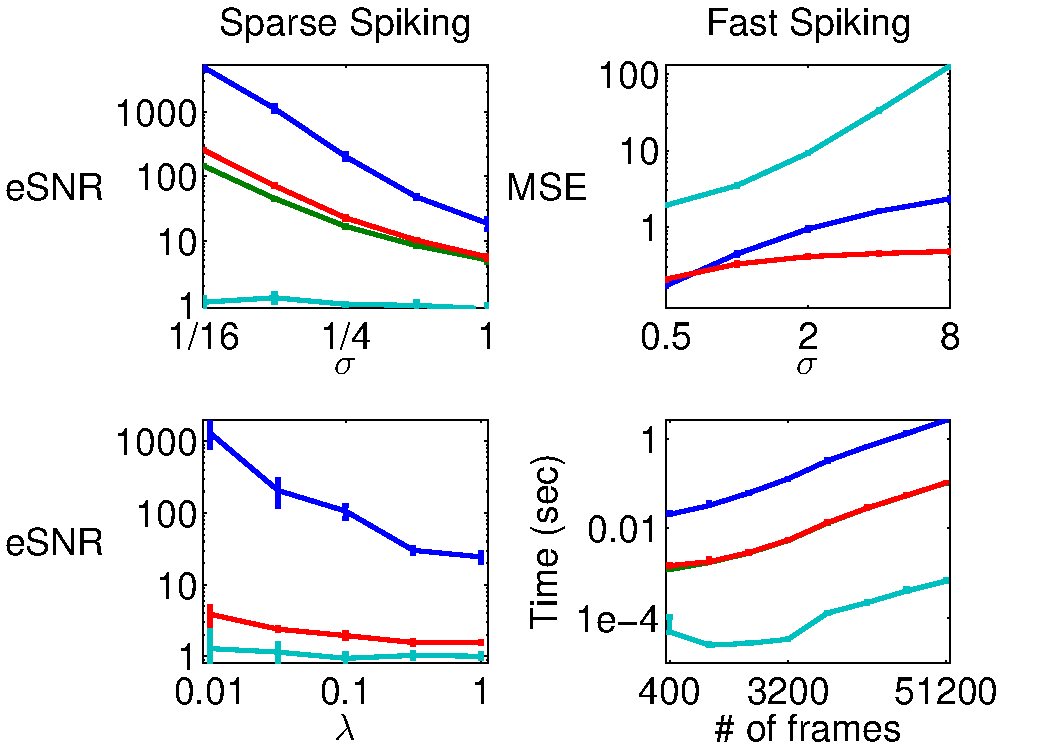
\includegraphics[width=.9\linewidth]{../figs/stats}
\caption{} \label{fig:stats}
\end{figure}


% To quantify the relative quality of these inference algorithms, Table \ref{tab:1} shows $R_{\hbn}$ and AUC for simulations like these, as well as computational time.  Clearly, the FAND filter is preferable to the Wiener filter, in that the FAND filter's performance is at least as good as the Wiener filter's, and requires less time.  
% 
% \begin{table}
% \caption{Simulated performance} \label{tab:slow}
% \centering
% \begin{tabular}{c|c|c|c|c|c}
% \multicolumn{6}{c}{Slow Firing Rate} \\ %\hline
% %Filter 			& $R_{\hbn}$ 	& $MSE$ 		& $SNR$ 		& $AUC$ & Time \\ \hline
% Filter & $R_{\hbn}$ & $MSE$ & $SNR$ & $AUC$ & Time \\ \hline 
FAND& 0.920 (0.009) & 0.006 (0.001) & 396.256 (91.462) & 6.315 (0.289) & 0.495 (0.020) \\ 
Wiener& 0.552 (0.012) & 0.024 (0.002) & 19.337 (1.508) & 6.485 (0.462) & 0.022 (0.001) \\ 
$[$Wiener$]_+$& 0.670 (0.010) & 0.017 (0.001) & 29.801 (2.436) & 6.485 (0.462) & 0.022 (0.001) \\ 
dF/F& -0.029 (0.009) & 0.067 (0.006) & 1.109 (0.222) & 0.853 (0.089) & 0.000 (0.000)
% %\end{tabular}
% %\end{table}
% \\ \hline \\
% %\begin{table}
% %\caption{Fast Firing Rate} \label{tab:fast}
% %\centering
% %\begin{tabular}{c|c|c|c|c|c}
% \multicolumn{6}{c}{Fast Firing Rate} \\ %\hline
% %Filter 			& $R_{\hbn}$ 	& $MSE$ 		& $SNR$ 		& $AUC$ & Time \\ \hline
% Filter & $R_{\hbn}$ & $MSE$ & $SNR$ & $AUC$ & Time \\ \hline 
FAND& 0.752 (0.005) & 67.689 (1.703) & NaN (NaN) & NaN (NaN) & 0.765 (0.016) \\ 
Wiener& 0.916 (0.001) & 15.323 (0.141) & NaN (NaN) & NaN (NaN) & 0.243 (0.005) \\ 
$[$Wiener$]_+$& 0.916 (0.001) & 15.323 (0.141) & NaN (NaN) & NaN (NaN) & 0.243 (0.005) \\ 
dF/F& 0.006 (0.005) & 385.433 (2.399) & NaN (NaN) & NaN (NaN) & 0.000 (0.000)
% \end{tabular}
% % }
% % \end{multicols}
% \end{table}

Finally, often one is interested in understanding the relationship between spike trains and the environment.  Therefore, we simulated a neuron whose spiking activity was a function of a 5-dimensional external stimulus.  More specifically, we let $\blam = \bk\T \bx$, where $\bk$ is a 5-dimensional linear kernel, and $\bx = (\bx_1, \ldots, \bx_T)$ is the stimulus, and $P(n_t)=$Poisson($\lam_t \Del$).  We then computed the maximum likelihood estimate of the linear kernel, $\hbk=\hbn \bx\T (\bx \bx\T)^{-1}$.  Importantly, the simulation was constructed to incorporate both sparse spiking and fast spiking periods, much like sensory neurons have periods of quiescence, followed by stimulus driven bursts.  Thus, neither the FAND filter nor the Wiener filter's assumptions are entirely appropriate. Figure \ref{fig:kernel} shows the results of this simulation.  The true kernel, kernel estimated using the true spike times, and kernel estimated using the FAND filter, are nearly overlapping (black, gray, and blue lines, respectively).  The kernel estimated using the Wiener filter output, however, is effectively flat (red line). Post-hoc half-wave rectification of the Wiener filter output does not improve its ability to estimate this kernel (green line --- completely obscured by the unrectified Wiener filter output).  Finally, dF/F does not yield anything useful at all (turquoise line).  

\begin{figure}[H]
\centering 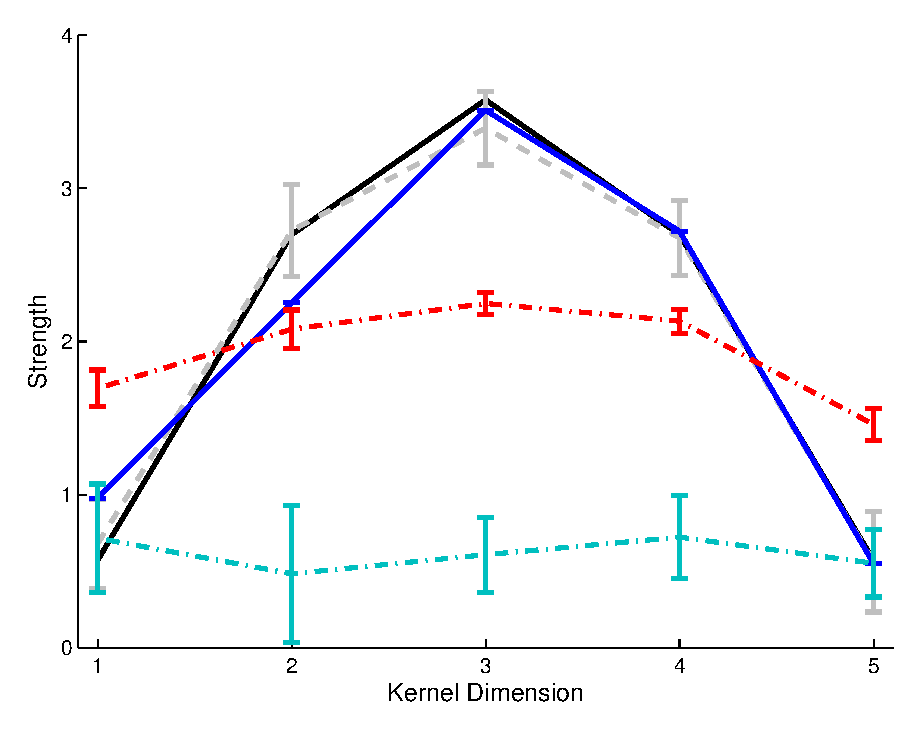
\includegraphics[width=.9\linewidth]{../figs/kernel}
\caption{XXX. Parameters: $T=800$, $\Del=5$ msec, $\alpha=1$, $\beta=0$, $\tau=100$ msec, $x_{i,t} \sim \mU(0,0.2)$,  $\sig=1/4$.} \label{fig:kernel}
\end{figure}


%The correlation coefficient between $\bn_{FAND}$ and $\bn$ versus $\bn_{Wiener}$ and $\bn$ for this example is $0.92$ versus $0.57$.  Thresholding $\bn_{Wiener}$ after inference improves the correlation coefficient to $0.69$.  Running this simulation many times demonstrates that these results are typical: $\bn_{FAND}$ always outperforms $\bn_{Wiener}$, whether or not it $\bn_{Wiener}$ thresholded.  

